%%%%%%%%%%%%%%%%%%%%%%%%%%%%%%%%%%%%%%%%%
% University/School Laboratory Report
% LaTeX Template
% Version 3.1 (25/3/14)
%
% This template has been downloaded from:
% http://www.LaTeXTemplates.com
%
% Original author:
% Linux and Unix Users Group at Virginia Tech Wiki 
% (https://vtluug.org/wiki/Example_LaTeX_chem_lab_report)
%
% License:
% CC BY-NC-SA 3.0 (http://creativecommons.org/licenses/by-nc-sa/3.0/)
%
%%%%%%%%%%%%%%%%%%%%%%%%%%%%%%%%%%%%%%%%%

%----------------------------------------------------------------------------------------
%	PACKAGES AND DOCUMENT CONFIGURATIONS
%----------------------------------------------------------------------------------------

\documentclass{article}

\usepackage[version=3]{mhchem} % Package for chemical equation typesetting
%\usepackage{siunitx} % Provides the \SI{}{} and \si{} command for typesetting SI units
\usepackage{graphicx} % Required for the inclusion of images
\usepackage{natbib} % Required to change bibliography style to APA
\usepackage{amsmath} % Required for some math elements 
\usepackage{hyperref}
 \usepackage{pdflscape}
\usepackage[a4paper,margin=0.5in]{geometry}
\setlength\parindent{0pt} % Removes all indentation from paragraphs

\renewcommand{\labelenumi}{\alph{enumi}.} % Make numbering in the enumerate environment by letter rather than number (e.g. section 6)

%\usepackage{times} % Uncomment to use the Times New Roman font

%----------------------------------------------------------------------------------------
%	DOCUMENT INFORMATION
%----------------------------------------------------------------------------------------

\title{Gate Detection} % Title

\author{Philipp \textsc{Duernay}} % Author name

\date{\today} % Date for the report

\begin{document}
\maketitle
% If you wish to include an abstract, uncomment the lines below
% \begin{abstract}
% Abstract text
% \end{abstract}

%----------------------------------------------------------------------------------------
%	SECTION 1
%----------------------------------------------------------------------------------------

\section{Recap}
In the last meeting from 28.05.2018 several next steps were defined:
\begin{itemize}
	\item Investigate speed/performance bottlenecks
\end{itemize}


\section{Performance/Speed Analysis}

I managed to run models on the camera and did some measurements on the inference time. Also I compared the performance at different amount of layers and resolutions. Results see next page.

\begin{figure}
	\begin{minipage}{0.5\textwidth}
		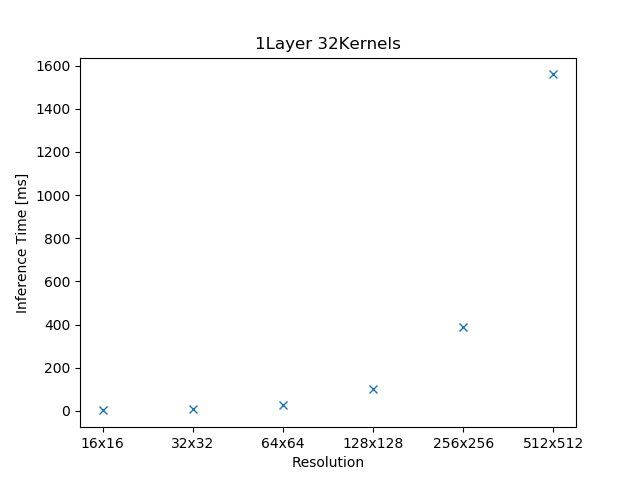
\includegraphics[width=\textwidth]{speed_res}
	\end{minipage}
	\begin{minipage}{0.5\textwidth}
	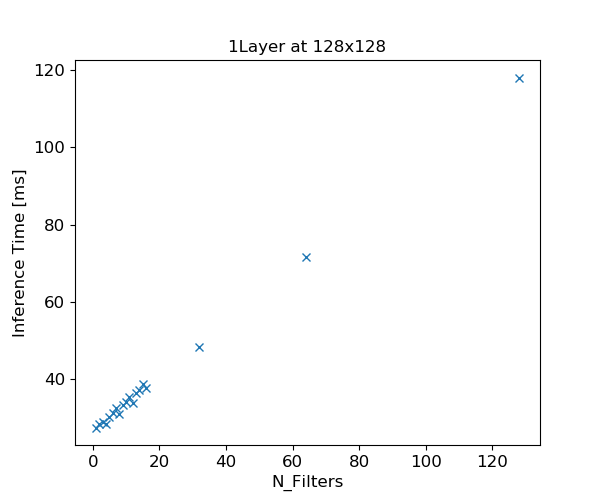
\includegraphics[width=\textwidth]{speed_width}
\end{minipage}

	\begin{minipage}{0.5\textwidth}
	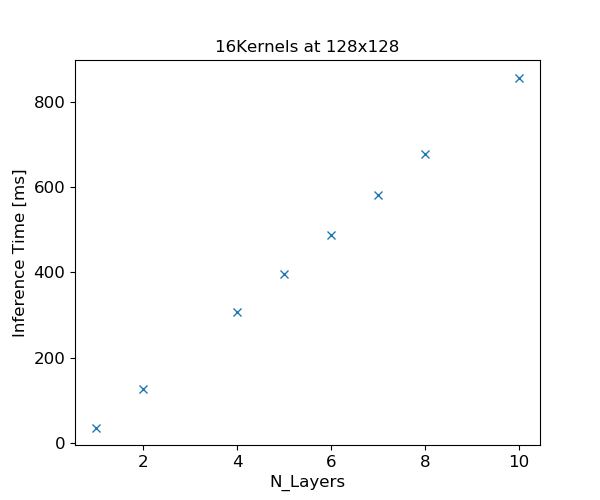
\includegraphics[width=\textwidth]{speed_layers}
\end{minipage}
\end{figure}


\begin{figure}
	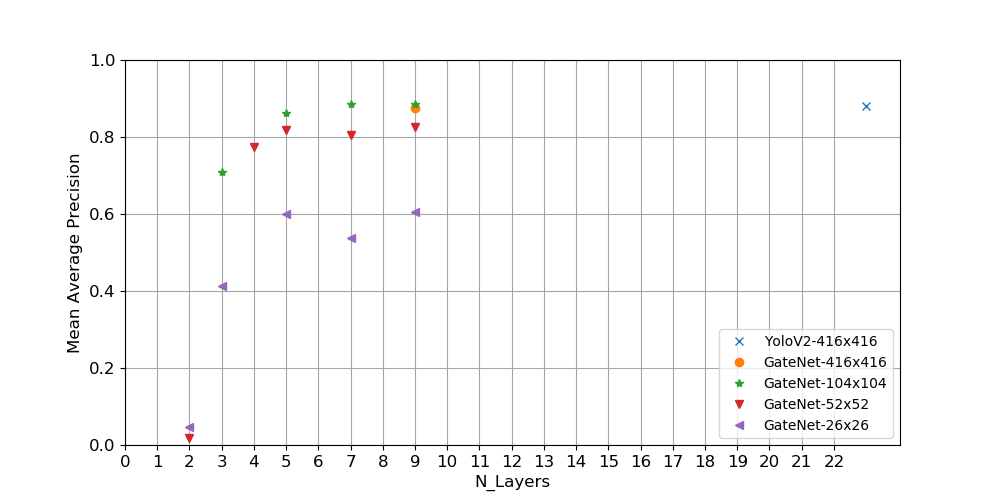
\includegraphics[width=\textwidth]{map_res_layers}
	\caption{Model Performance at different resolutions/architectures.}
\end{figure}


\section{Conclusion}
\begin{itemize}
	\item Time scales linearly with amount of pixels.
	\item Full resolution prohibitively slow.
	\item Increasing width quite cheap. ~1ms per kernel.
	\item Increasing layers expensive
	\item Reducing performance at first minor effect on detection
	\item If we want to achieve ~10Hz we can't have more than about 3 layers at 64x64
\end{itemize}

\section{Next Steps}
\begin{itemize}
	\item Investigate effect of quantization on performance and speed
	\item Investigate effect of depthwise separable convolutions on performance and speed
	\item Reduce final grid of model
	\item 1 Model that predicts a region to crop in the next frame, 1 Model that finds corners?
\end{itemize}

\newpage
\appendix

\begin{table}[htbp]
	\caption{}
	\begin{tabular}{|l|r|r|r|r|r|r|r|r|}
		\hline
		Resolution/Model & \multicolumn{1}{l|}{Conv\_w32\_6x6→Pool→Norm} & \multicolumn{1}{l|}{} & \multicolumn{1}{l|}{Conv\_w1\_3x3} & \multicolumn{1}{l|}{} & \multicolumn{1}{l|}{Pool2x2} & \multicolumn{1}{l|}{} & \multicolumn{1}{l|}{Norm} & \multicolumn{1}{l|}{} \\ \hline
		16x16 & 1.91 & 0.26 & 1.36 & 0.22 & 0.06 & 0.06 & 0.03 & 0.03 \\ \hline
		32x32 & 7.06 & 1.13 & 5.02 & 0.03 & 0.18 & 0.12 & 0.1 & 0.12 \\ \hline
		64x64 & 26.95 & 0.31 & 10.22 & 0.15 & 0.7 & 0.2 & 0.4 & 0.22 \\ \hline
		128x128 & 99.75 & 1.67 & 25.3 & 0.82 & 2.7 & 0.18 & 1.5 & 0.23 \\ \hline
		256x256 & 390.62 & 48.8 & 88.6 & 1.31 & 11.7 & 0.2 & 6.12 & 0.12 \\ \hline
		512x512 & 1559.67 & 280.85 & 352.01 & 10.34 & 47.98 & 0.12 & 24.5 & 0.25 \\ \hline
	\end{tabular}
	\label{}
\end{table}

\begin{table}[htbp]
	\caption{}
	\begin{tabular}{|r|r|r|}
		\hline
		\multicolumn{1}{|l|}{Filter Size} & \multicolumn{1}{l|}{Conv\_wX\_3x3\_pool2x2\_norm\_128x128} & \multicolumn{1}{l|}{} \\ \hline
		1 & 27.49 & 0.93 \\ \hline
		2 & 28.45 & 0.12 \\ \hline
		3 & 29 & 0.04 \\ \hline
		4 & 28.36 & 0.22 \\ \hline
		5 & 30.3 & 0.23 \\ \hline
		6 & 31.18 & 0.12 \\ \hline
		7 & 32.55 & 0.23 \\ \hline
		8 & 30.88 & 0.08 \\ \hline
		9 & 33.41 & 0.23 \\ \hline
		10 & 34.14 & 0.13 \\ \hline
		11 & 35.4 & 0.23 \\ \hline
		12 & 33.85 & 0.1 \\ \hline
		13 & 36.5 & 0.24 \\ \hline
		14 & 37.24 & 0.2 \\ \hline
		15 & 38.72 & 0.28 \\ \hline
		16 & 37.66 & 0.28 \\ \hline
		32 & 48.44 & 0.28 \\ \hline
		64 & 71.58 & 0.8 \\ \hline
		128 & 118.08 & 0.47 \\ \hline
	\end{tabular}
	\label{}
\end{table}

\begin{table}[htbp]
	\caption{}
	\begin{tabular}{|r|r|r|}
		\hline
		\multicolumn{1}{|l|}{Layers} & \multicolumn{1}{l|}{Conv\_w16\_3x3\_pool2x2\_norm\_128x128} & \multicolumn{1}{l|}{} \\ \hline
		1 & 36.6 & 0.37 \\ \hline
		2 & 126.52 & 0.58 \\ \hline
		3 & \multicolumn{1}{l|}{} & \multicolumn{1}{l|}{} \\ \hline
		4 & 306.48 & 3.8 \\ \hline
		5 & 396.45 & 1.42 \\ \hline
		6 & 486.6 & 3.92 \\ \hline
		7 & 580.43 & 86.51 \\ \hline
		8 & 677.7 & 256.46 \\ \hline
		9 & \multicolumn{1}{l|}{} & \multicolumn{1}{l|}{} \\ \hline
		10 & 856.36 & 345.06 \\ \hline
	\end{tabular}
	\label{}
\end{table}


%----------------------------------------------------------------------------------------
\bibliographystyle{abbrv}

\bibliography{literature}

%----------------------------------------------------------------------------------------


\end{document}\grid
